%!TEX root = ../thesis.tex

\section {Criptografia en Blockchain}  %Title of the First Chapter

%\textcolor{red}{Me parece que el término correcto es crifra, en lugar de encriptar. Verificar.}
%\textcolor{blue} {encriptar cambiado por cifrar en varias partes del parrafo, verificar si es la correcion sugerida. Link de referencia: http://red.computerworld.es/actualidad/cuando-alguien-dice-encriptar-y-quiere-decir-cifrar}

La criptografía es la ciencia encargada del estudio de los algoritmos, protocolos y sistemas que se utilizan para dotar de seguridad a las comunicaciones, a la información y a las entidades que se comunican~\cite{pastor1998criptografia}.

El método en general implica tomar datos sin cifrar, como una pieza de texto, y cifrarlos usando un algoritmo matemático. Esto produce un texto cifrado, una información que es completamente inútil y sin sentido, hasta que se descifra con la ayuda de una clave preestablecida y conocida solamente por el emisor y receptor. Este método  criptográfico se conoce como criptografía de llave simétrica (ver Figura~\ref{blockcain_llavesimetrica}).

\begin{figure}[h]
    \centering
    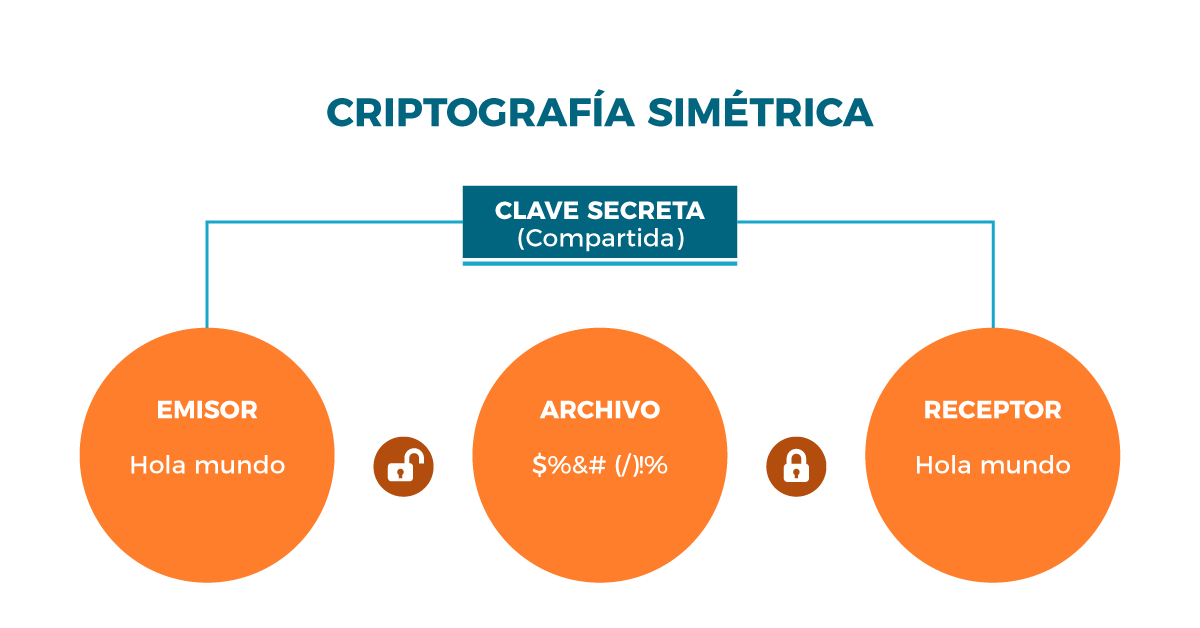
\includegraphics[width=0.7\textwidth]{cripto_simetrica.png}
     \caption{Método criptografico de llave simétrica} 
    \label{blockcain_llavesimetrica}
\end{figure}

La criptografía proporciona varios servicios de seguridad, los cuales son vitales y necesarios en tecnología \textit{blockchain} o cualquier plataforma que haga uso de la misma~\cite{bashir2017mastering}:

\begin{itemize}
    \item \textbf{Confidencialidad} es la garantía de que la información solo está disponible para las entidades autorizadas.
    \item \textbf{Integridad} es la garantía de que la información es modificable sólo por entidades autorizadas.
    \item \textbf{Autenticación} proporciona seguridad sobre la identidad de una entidad o la validez de un mensaje. Hay dos tipos de autenticación:
    La \textbf{autenticación de la entidad} es la garantía de que una entidad está actualmente involucrada y activa en una sesion de comunicacion.
    La \textbf{autenticación de origen de datos}  es la garantía de verificación sobre la fuente de información, esta  implica la integridad de los datos ya que si  una fuente ha sido corroborada, se asegura que los datos no han sido alterados. Diversos métodos, como los códigos de autenticación de mensajes (MAC, por sus siglas en ingles  Message Authentication Code) y las firmas digitales son los más comúnmente utilizados.
    \item \textbf{No repudio}  es la  garantía de que una entidad no puede negar un compromiso o acción previa proporcionando evidencia. El uso de criptografía garantiza que este servicio produce evidencias infalibles e irrefutables  en transacciones electrónicas para que, en caso de disputas, se pueda utilizar como confirmación de una acción.
    \item \textbf{Rendición de Cuentas} es la garantía de que las acciones que afectan la seguridad de la plataforma se pueden rastrear hasta la fuente responsable. Esto generalmente es proporcionado por los mecanismos de registro y auditoría en los sistemas donde se requiere una auditoría detallada debido a la naturaleza del negocio.
\end{itemize}
 
\subsection {Criptografía de llave pública}

A pesar de estar basado en un marco similar, el tipo de criptografía utilizado en \textit{blockchain} es conocida como \textbf{criptografía de llave pública} o \textbf{criptografía asimétrica}, este tipo representa una mejora en la criptografía de llave simétrica estándar, ya que permite que la información se transfiera a través de una llave pública que se puede compartir con cualquier persona~\cite{liskacademy:blockchainCryptographyExplained}.

En la práctica el remitente cifra los datos usando la llave pública del destinatario y luego los transmite a través de la red al receptor. Una vez que llega al receptor, se puede descifrar usando la llave privada del receptor. De esta manera, la llave privada permanece en el lado del receptor y no hay necesidad de compartir llaves para realizar el cifrado y descifrado, que es lo que ocurre en el cifrado simétrico. La Figura~\ref{blockcain_llaveasimetrica} muestra gráficamente este proceso.

Adicionalmente, a través de la criptografía de llave pública se produce una firma digital que garantiza la integridad de los datos que se muestran. Esto se hace combinando la llave privada de un usuario con los datos que desean firmar, a través de un algoritmo matemático.

\begin{figure}[h]
    \centering
    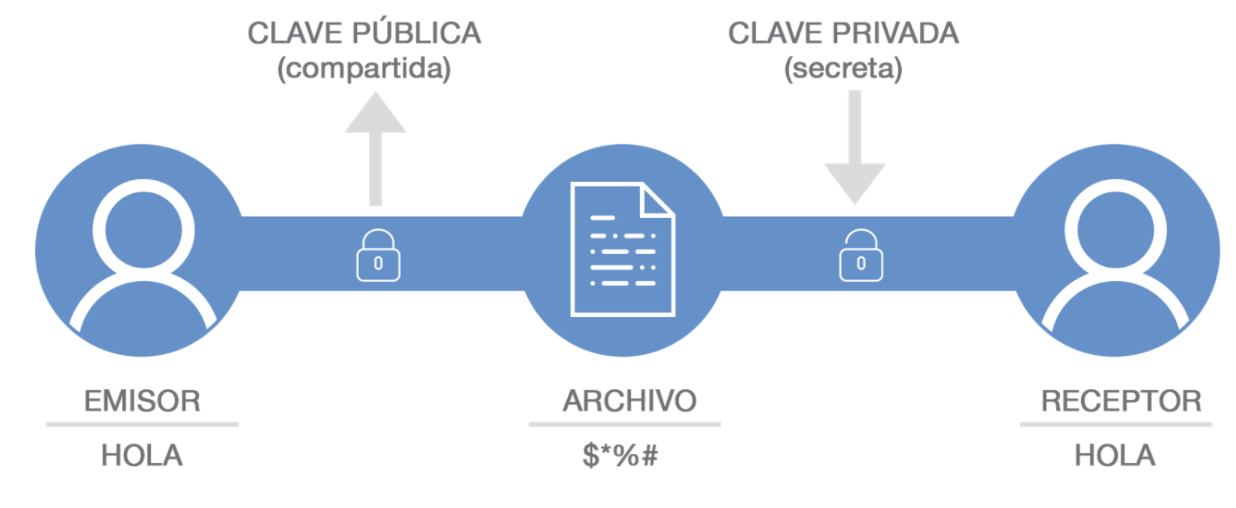
\includegraphics[width=0.7\textwidth]{cripto_asimetrica.png}
     \caption{Método criptográfico de llave asimétrica} 
    \label{blockcain_llaveasimetrica}
\end{figure}

\subsection{Firmas digitales}

Las firmas digitales proporcionan un medio para asociar un mensaje con una entidad desde la cual se originó . Las firmas digitales se usan para proporcionar integridad, autenticación de origen de datos y no repudio.

Dentro de las firmas digitales encontramos 3 propiedades importantes a resaltar, la autenticidad, imposibilidad de force y la no reutilización. Autenticidad significa que las firmas digitales son verificables por una parte receptora. La  imposibilidad de force garantiza que solo el remitente del mensaje pueda usar la funcionalidad de firma con la llave privada y finalmente la no reutilización significa que la firma digital no se puede separar de un mensaje para ser utilizado en otro distinto.

Las firmas digitales son creadas a partir de tres algoritmos cuya finalidad radica en 
hacer absolutamente imposible calcular la llave privada en función de la clave pública o de los datos cifrados y garantizar la autenticidad de una firma basada en el mensaje y la llave privada, verificada a través de la clave pública. A continuación  se describen brevemente los algoritmos:
\begin{itemize}
    \item Un algoritmo de generación de claves, que proporciona una llave privada y pública.
    \item Un algoritmo de firma que combina datos y llave privada para hacer una firma.
    \item Un algoritmo que verifica las firmas y determina si el mensaje es auténtico o no en función del mensaje, la clave pública y la firma.
\end{itemize}

\subsection{Hashing}

Hashing es el proceso de tomar una entrada de cualquier longitud y convertirla en una salida criptográfica fija a través de un algoritmo matemático (Bitcoin usa SHA-256, por ejemplo). Los ejemplos de tales entradas pueden incluir desde un pequeño fragmento de información, como un mensaje hasta un gran caché de información variable, como un bloque de transacciones~\cite{liskacademy:blockchainCryptographyExplained}. La Figura~\ref{blockcain_hashing} ilustra el mecanismo de hashing.

\begin{figure}[h]
    \centering
    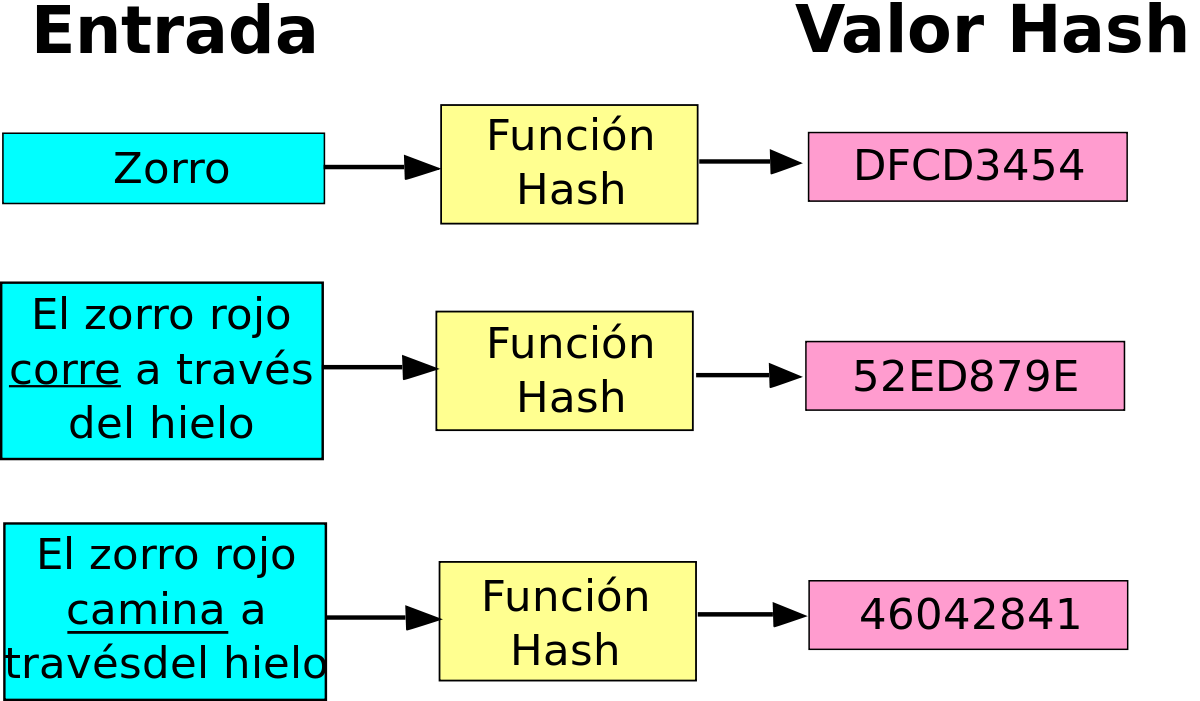
\includegraphics[width=0.6\textwidth]{hashing.png}
     \caption{Ilustración de mecanismo hashing} 
    \label{blockcain_hashing}
\end{figure}

El hashing aumenta drásticamente la seguridad de los datos ya que cualquiera que intente descifrar los datos mirando  el código  hash no podrá calcular la longitud de la información cifrada en función del hash mencionado. Una función de hash criptográfica debe tener varias cualidades cruciales para ser considerada útil:
\begin{itemize}
    \item Imposible producir el mismo valor hash para diferentes entradas.
    \item El mismo mensaje siempre producirá el mismo valor hash.
    \item Rápido en  la  generacion de un hash para cualquier mensaje dado.
    \item Imposible determinar la entrada en función del valor hash.
    \item Incluso el más mínimo cambio a una entrada altera por completo el hash.
\end{itemize}

En \textit{blockchain}, los hashes se usan para representar el estado actual del mundo, o para ser más precisos, el estado del \textit{blockchain}. La entrada representa todo lo que ha sucedido en el \textit{blockchain}, es decir, cada transacción realizada hasta ese punto combinada con los nuevos datos que se agregan.

Como se mencionó, el más mínimo cambio en cualquier parte de la entrada da como resultado un gran cambio en la salida; en esto radica la seguridad irrefutable de la tecnología \textit{blockchain}. Cambiar cualquier registro que haya sucedido previamente en un \textit{blockchain} cambiaría todos los hashes, haciéndolos falsos y obsoletos. Esto se vuelve imposible cuando se toma en cuenta la naturaleza transparente de \textit{blockchain}, ya que estos cambios deberían realizarse a plena vista de toda la red y en todos los nodos que la conforman.

El primer bloque de una cadena de bloques, conocido como bloque de génesis, contiene sus transacciones que, cuando se combinan y validan, producen un hash único. Este hash y todas las transacciones nuevas que se están procesando se usan luego como entrada para crear un nuevo hash que se usa en el siguiente bloque de la cadena. Esto significa que cada bloque se vincula a su bloque anterior a través de su hash, formando una cadena de regreso al bloque de génesis, de ahí el nombre \textit{blockchain}. De esta forma, las transacciones se pueden agregar de forma segura siempre que los nodos de la red estén en consenso sobre cuál debería ser el hash.


